\section{Scenarios}


The obstruction-free fish-eye lens can be used with different types of volumetric datasets. First, we present a scenario based on baggage inspection (an heterogeneous dataset). Second, we apply our lens technique to a volume of streamlines where the transparency doesn't allow seeing a dense spherical item within its context. Finally, we observe  a special aircraft trajectory within its context inside a dataset representing one day of traffic.

\subsection{Baggage inspection: An unusual blunt object}

\begin{figure*} 
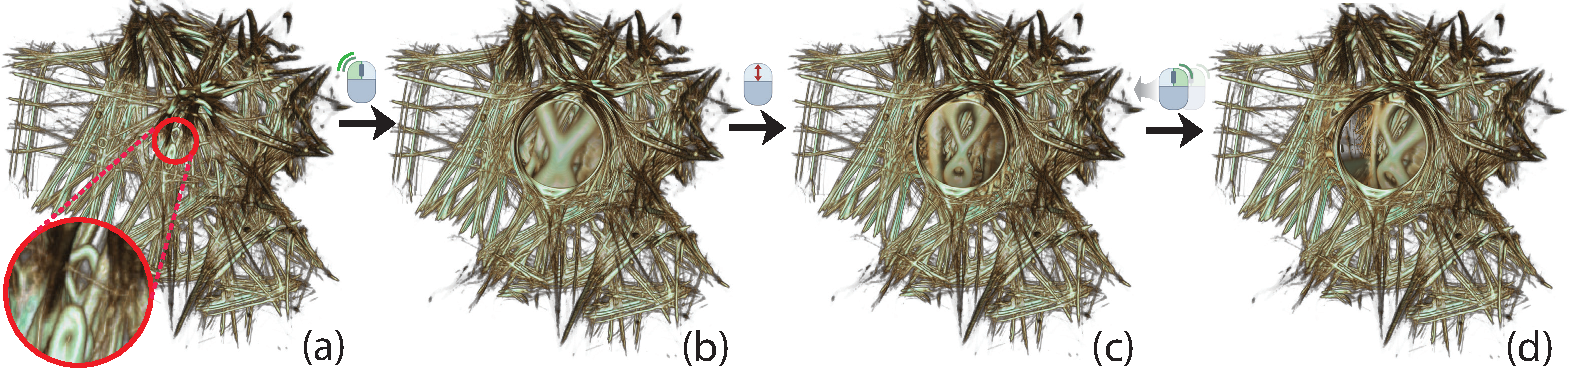
\includegraphics [width=\textwidth]{images/aircraft_lens.pdf} 
\caption{Inspecting an abnormal aircraft trajectory. (a) The initial view on the trajectories where the abnormal trajectory was spotted. (b) The transition  towards a magnified trajectory starts just after the lens tool has been used (double click). (c) The trajectories is magnified. (d) Local Rotations allow to look around the target (right click+ mouse drag toward the desired direction).}
\label{f:aircraft_lens}
\end{figure*}
In most airports, security agents deal with volumetric data exploration during baggage inspections. While automatic systems are now able to detect harmful densities (such as  C-4, TNT, Nitroglycerin, etc.) and event some prohibited articles (such as classical firearms and knives), it remains difficult to identify unusual threats. In addition, baggage inspection faces 4 main concealment strategies:

\textbf{Superposition}: A threat (e.g. prohibited object like a knife, a cutter…) may be sheltered behind dense materials. Sometimes, it’s possible to see through these blind shield using some functionalities such as high penetration (enhanced X-ray power) or image processing (contrast improvement). 

\textbf{Location}: Depending on its location inside the luggage, a threat can be difficult to detect. Objects located in the corners, in the edges or inside the luggage’s frame are very difficult to identify.

\textbf{Dissociation}: Another way to dissimulate a threat is to separate and to spread parts of it in the luggage (weapon or explosive are composed of many separated items like the trigger, the cannon...). This dissociation can be combined with other dissimulation techniques.

\textbf{Lure}: An ill-intentioned individual may use a lure to hide the real threat. For instance, a minor threat like a small scissors may be clearly visible and catch security agent’s attention while a more important threat remains hidden.

As an example, a baggage containing different types of objects as in \autoref{f:baggage_orientation} ( with a volume size of 283x189x344 ) can be declared non-suspect by automatic inspection systems. However, while exploring this baggage with different angles and perspectives, it appears that an object is hidden between a set of mugs. A common solution to this type of issue in baggage inspection is to filter the materials by density in order to show or hide subsets of the volume and reduce the occlusion. But in this case, trying to discriminate the materials on the basis of their densities is not enough to fully reveal the hidden object (\autoref{f:baggage_lens}b-d). In fact, this suspect item shares almost the same density as the surrounding ceramic mugs. 

Using the obstruction-free fish-eye lens can help in this kind of situation. The user has just to use this tool on the partially hidden target. Then, a transition inside the lens will start and smoothly provide the finale unobstructed view of the blunt object which is, in this case, a ceramic shuriken (\autoref{f:baggage_lens}e-g). 



\subsection{Fluid flow: A deep-buried spherical vortex}
\label{sec:flow}
%
%
Flow visualization using streamlines has a long history in scientific visualization~\cite{brambilla2012illustrative,xxx}. When applied to 3D datasets, a key challenge is to balance the streamline density. Low values allow seeing inner regions in the data but can subsample (miss) important patterns. High values show more data but create too much occlusion. We next show how our lens can be used to discover interesting patterns in the second case, \emph{i.e.}, a 3D volume densely filled with streamlines. The dataset, introduced in\,\cite{griebel2004flow}, captures the simulation of water flow in a basin computed on a grid of 128x85x42 cells. A set of 4595 streamlines with 183K sample points is next traced by pseudo-random seeding over this vector field. We convert this set of 3D curves (polylines) to a scalar volume by using kernel density estimation (KDE)\,\cite{silverman1986density}. Similar techniques have been used to compute density maps of 2D trail-sets\,\cite{hurter2012graph,cubu,hurter2015image}. To increase computational speed, we compute the KDE in the frequency space and using GPU acceleration, following\,\cite{lhuillier2017ffteb}. The resulting volumes have a resolution of $500^3$ voxels and can be directly displayed using DVR (\autoref{f:streamLineSTDViz}). Note that, given the smoothing effect of KDE, streamlines appear now as finite-thickness tubes rather than pixel-thin curves.

For a first overview, we display the volume using standard DVR. After turning the viewpoint a bit, we notice a dense spherical item inside the dataset (\autoref{f:streamLineSTDViz}a). To see its shape better, we increase the opacity; however, this immediately increases occlusion so the item becomes invisible. Conversely, decreasing opacity to reduce occlusion makes the item almost transparent. Our lens solves the problem: In the initial view (\autoref{f:streamLineSTDViz}a), we point at the object and turn on the lens. This effectively pushes away the occluding stream bundles, and lets us see that our item is nearly perfectly spherical (\autoref{f:stream_lens}). This is something we could not have assessed from \emph{any} viewpoint and with likely any opacity modulation using standard DVR. Our object is a set of densely-packed, low-speed, tightly-turning streamlines that create a ball-like vortex. Interestingly, this spherical vortex has not been discovered by any of the visualization techniques that we are aware of that used this same dataset\,\cite{telea_vis_99,griebel2004flow,ddh,lhuillier2017ffteb,maybe_more}.


\begin{figure*}[htb]
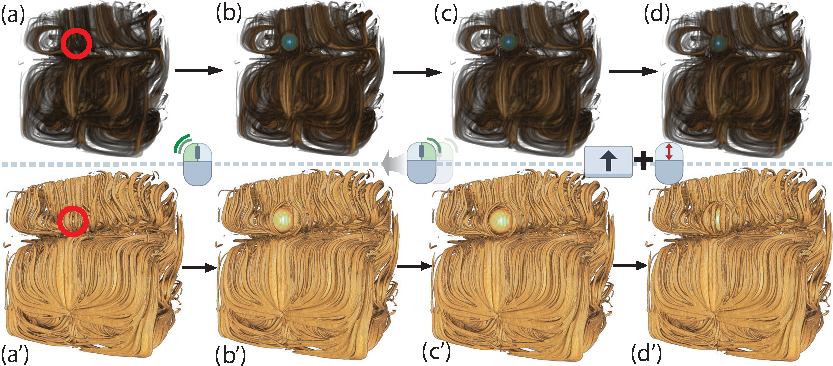
\includegraphics [width=\textwidth]{images/stream_lens.pdf}
\caption{A spherical item and its surrounding area are inspected using to our lens with two different transfer functions. The first part is displayed with transparency in opposition to the part below. The opacity helps to see the shape of the surrounding whirlpool. (a-a') The streamline dataset displayed using our framework. A dense object is hidden inside a whirlpool. (b-b') The lens tool is applied to the partially hidden object (double-click). The area is magnified and the occluding part of the whirlpool located in front of the spherical item is pushed aside. (c-c') The directions of the rays inside the lens are modified to see the whole sphere through the lens (right click+ mouse drag toward the desired direction). (d-d') The occluding part of the whirlpool can be restored/pushed gradually while keeping the area magnified (Shift + scroll).  }
\label{f:stream_lens}
\end{figure*}

\begin{figure}[htb]
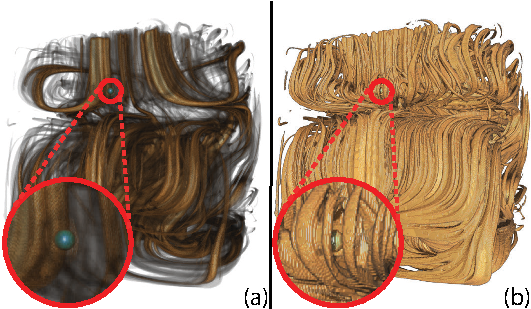
\includegraphics [width=0.45\textwidth]{images/streamline_orientation.pdf}
\caption{Two views of a streamlines dataset. (a) The transfer function used allows to spot a spherical dense item inside the volume thanks to transparency. (b) This spherical object become occluded when the opacity of the surrounding whirlpool is increased in order to analyze its shape and behavior. \textbf{ALEX: Could and should be merged with \autoref{f:stream_lens}.}}
\label{f:streamLineSTDViz}
\end{figure}


\subsection{Aircraft trajectories: Outliers in the French sky}
%
%
One of the major issue when visualizing large dataset of moving object is to address the occlusion issue where too many lines spoil their investigation. Many investigations have already been done, especially regarding aircraft movement exploration \cite{hurter2014interactive}.
\begin{figure} 
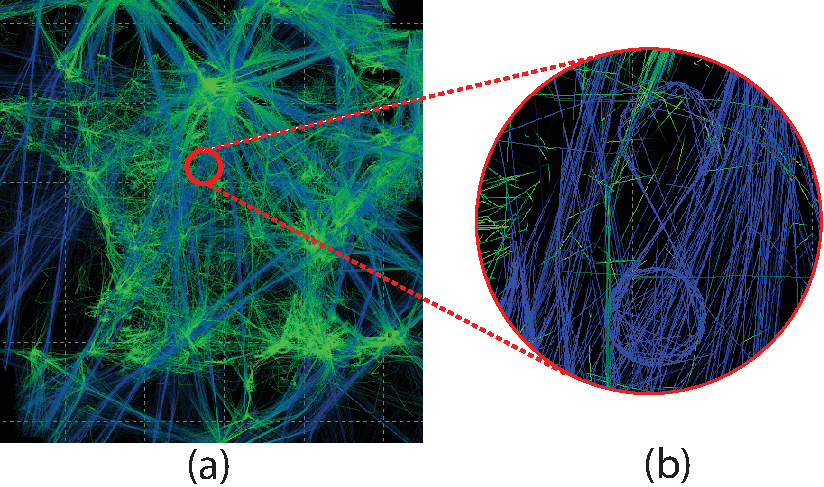
\includegraphics [width=0.45\textwidth]{images/aircraft.pdf} 
\caption{ Standard visualization of one day of recorded aircraft trajectories over France.\cite{hurter2009fromdady}. (a) An unusual trajectory is spotted but needs some manipulation to be unobstructed. (b) Zoom and color filtering technique to visualize abnormal trajectory of one aircraft performing a loop with an eight shape trajectory. This aircraft corresponds to a tanker waiting for refueling other aircraft.}
\label{f:fromdady}
\end{figure}
Figure \autoref{f:fromdady}-a shows one day of recorded aircraft trajectories and \autoref{f:fromdady}(b) shows a subset of such dataset where one can visualize an abnormal aircraft trajectory. A tanker aircraft performed an eight shape loop while waiting to refuel other aircraft. Even if the visualization of such specific trajectory is possible with existing tools, it remains a difficult task which requires time and complex settings. With our technique (with a volume size of 500x500x500), the user can easily spot the corresponding aircraft and even if this trajectory remains barely visible, our lens tools will remove the occluding trajectory thus providing a suitable point of view to fully investigate this trajectory. Furthermore, this obstruction free lens allows to look around the targeted trajectory in order to look for neighboring trajectories.

\begin{figure} 
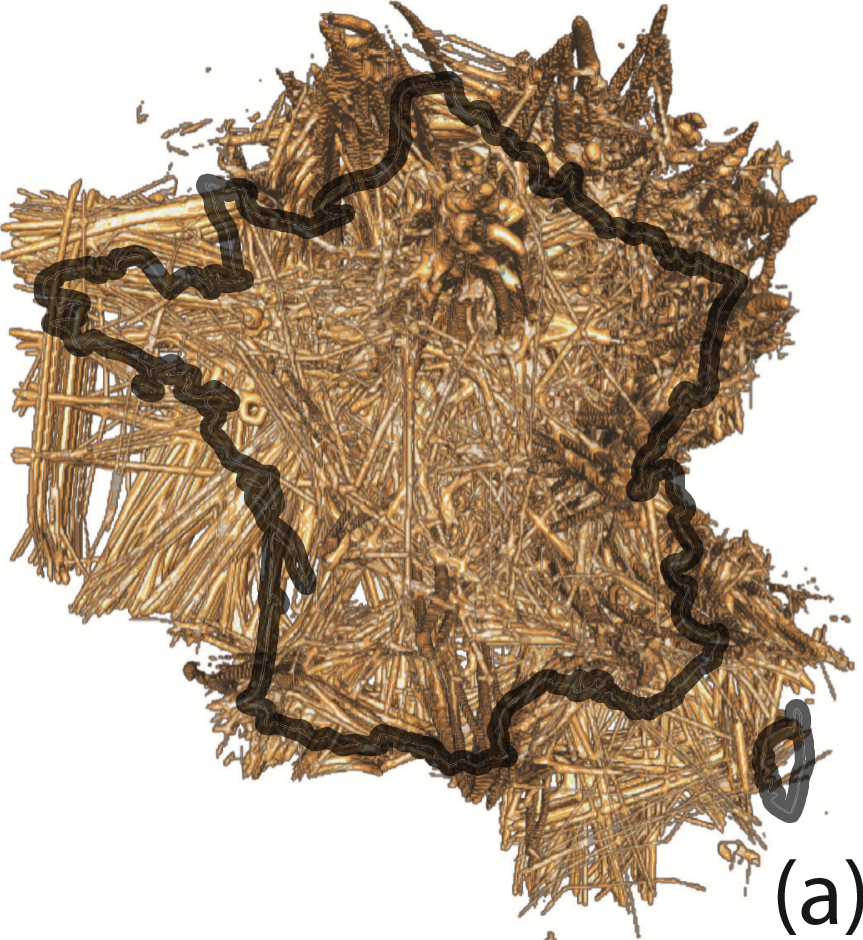
\includegraphics [width=0.36\textwidth]{images/topViewFR.png} 
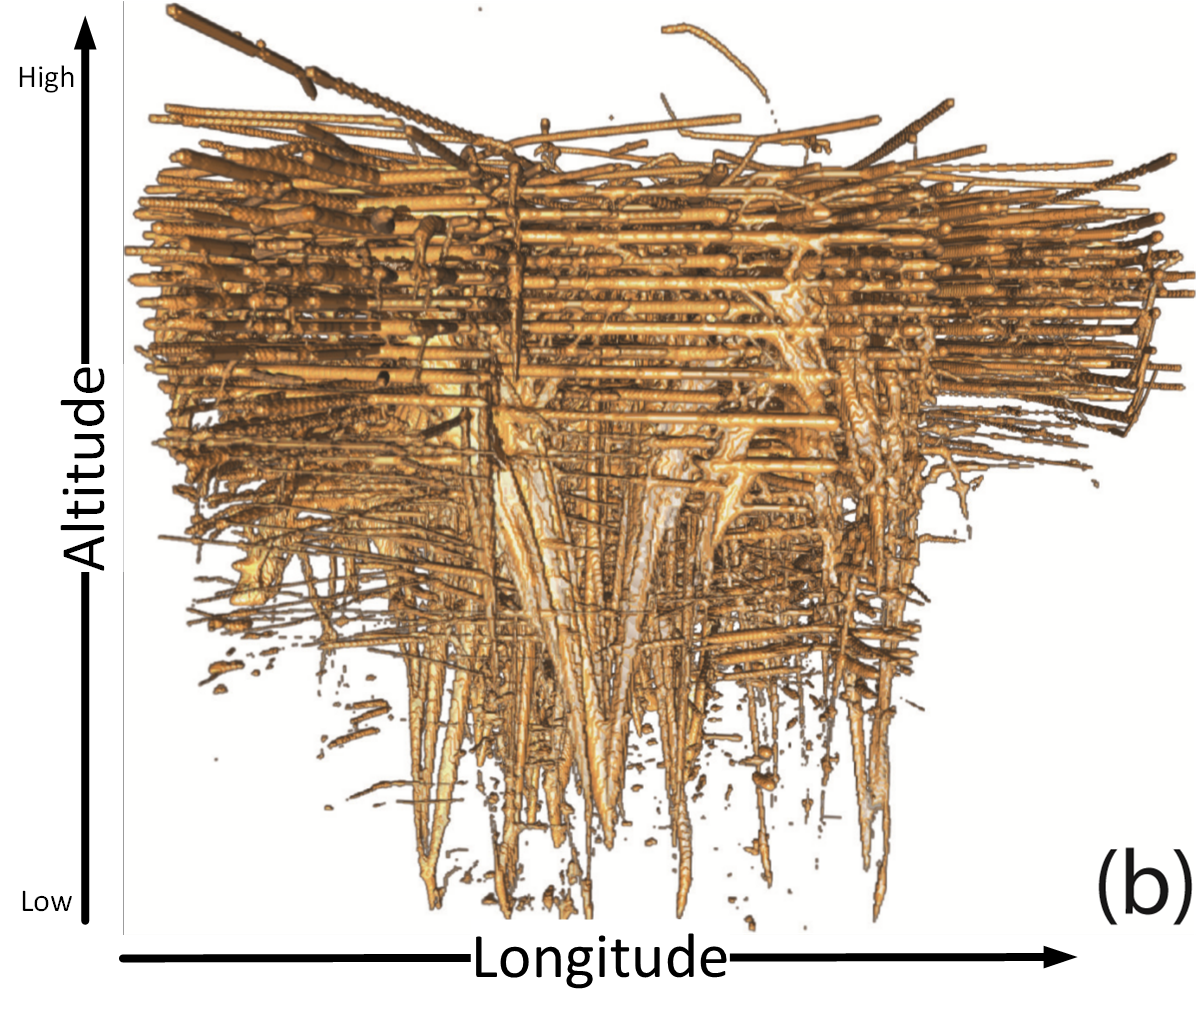
\includegraphics [width=0.4\textwidth]{images/VerticalViewLabel.png} 
\caption{Visualization of one day of recorded aircraft trajectories over France using our volume rendering framework. (a) The trajectories almost draw the map of France. (b) The trajectories are displayed according to their altitudes. }
\label{f:aircraft_orientation}
\end{figure}


